\section{Лекция 15.\\ Подтипы.}

\subsection{Система типов \(F_{<:}\)}

Мы рассматривали параметрический полиморфизм, как в системе типов Хиндли-Милнера. Но есть и другой подход --- ООП. Построим систему типов, которая описывает ООП, назовём её \(F_{<:}\). Определим отношение \(<:\) на типах, которое будет значить \(F <: G \Leftrightarrow\) если \(f : F, g : G\), то \(f\) годится везде, где годится \(g\).

Рассмотрим типы \(T = F \to H, S = G \to H, T' = H \to F, S' = H \to G\), где \(F <: G\). Тогда:
\begin{itemize}
    \item \(S <: T\), потому что функция \(S\) принимает в качестве аргумента \(G\), следовательно, она примет и \(F\)
    \item \(T' <: S'\), потому что возвращенный функцией \(T'\) элемент типа \(F\) подойдёт куда угодно, куда и возвращенный функцией \(S'\) элемент типа \(G\).
\end{itemize}

\begin{figure}[h]
    \centering
    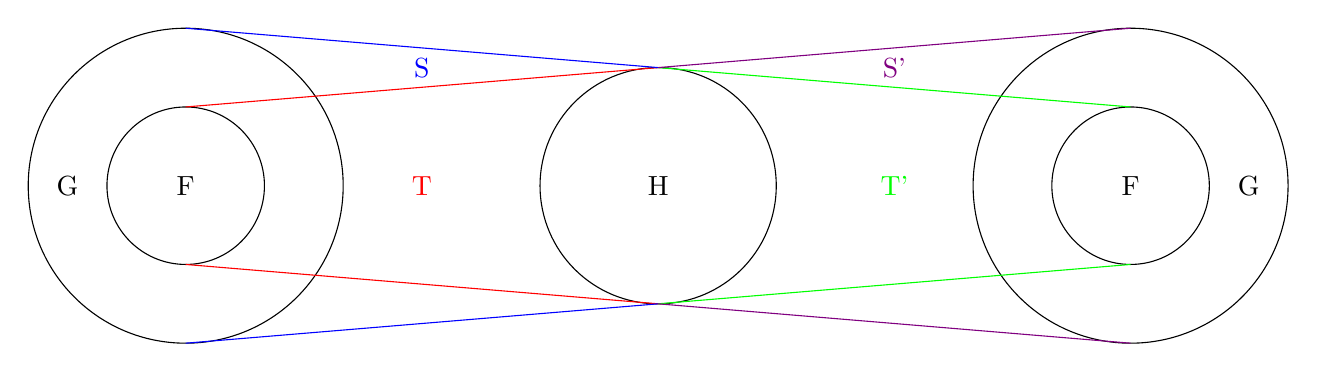
\begin{tikzpicture}
        \node at (-3, 0) {F};
        \node at (-4.5, 0) {G};
        \draw (-3, 0) circle (2 cm);
        \draw (-3, 0) circle (1 cm);
        \draw (3, 0) circle (1.5 cm);
        \node at (3, 0) {H};
        \draw[red] (-3, 1) -- (3, 1.5);
        \draw[red] (-3, -1) -- (3, -1.5);
        \draw[blue] (-3, 2) -- (3, 1.5);
        \draw[blue] (-3, -2) -- (3, -1.5);
        \node[red] at (0, 0) {T};
        \node[blue] at (0, 1.5) {S};
        \draw (9, 0) circle (2 cm);
        \draw (9, 0) circle (1 cm);
        \node at (9, 0) {F};
        \node at (10.5, 0) {G};
        \draw[green] (3, 1.5) -- (9, 1);
        \draw[green] (3, -1.5) -- (9, -1);
        \draw[violet] (3, 1.5) -- (9, 2);
        \draw[violet] (3, -1.5) -- (9, -2);
        \node[green] at (6, 0) {T'};
        \node[violet] at (6, 1.5) {S'};
    \end{tikzpicture}
\end{figure}

\begin{definition}
    Рассмотрим направленный граф \(F\). Отображение графов \(f : F \to G\) называется \textbf{ковариантным}, если \(a \prec_F b \Rightarrow f(a) \prec_G f(b)\) и \textbf{контравариантным}, если \(a \prec_F b \Rightarrow f(a) \succ_G f(b)\), где \(\prec_A\) --- отношение направленной инцидентности в графе \(A\). Это можно рассмотреть с точки зрения теории категорий, тогда \(F, G\) --- категории, \(f\) --- функтор.
\end{definition}

Несложно заметить, что отображение \(x \mapsto x \to H\) контравариантно, а отображение \(x \mapsto H \to x\) ковариантно на графе типов с ребрами, индуцированными отношением \(<:\).

\begin{example}
    Рассмотрим массив \(\texttt{[]}: * \to *\). Есть два метода "--- \texttt{get} и \texttt{set}. Так как один ковариантен, а другой контравариантен, получается, что если \(A <: B\), то и \(A\texttt{[]} <: B\texttt{[]}\), и \(B\texttt{[]} <: A\texttt{[]}\), следовательно, массив инвариантен (ковариантен и контравариантен одновременое).
\end{example}

В java ковариантность и контравариантность выражается через \texttt{super} и \texttt{extends}.

\subsection{Формализация \(F_{<:}\)}

Введём символ \(S <: T\) и правила вывода:
\begin{enumerate}
    \item \(\infer[\text{рефлексивность}]{S <: S}{}\)
    \item Введём тип \(\mathrm{Top}\)\footnote{В java это \texttt{Object}}. \(\infer[\text{рефлексивность}]{S <: \mathrm{Top}}{}\)
    \item \(\infer[\text{транзитивность}]{S <: T}{
              S <: U & U <:T
          }\)
    \item \(\infer[\text{ко- и контравариантность}]
          {S_1 \to S_2 <: T_1 \to T_2}
          {T_1 <: S_1 & S_2 <: T_2}\)
    \item Все правила для \(\lambda_{\to}\).
    \item \(\infer{\Gamma \vdash t : T}{\Gamma \vdash t : S & S <: T}\) --- связь между \(\lambda_{\to}\) и \(<:\).
\end{enumerate}

Рассмотрим функцию \(\Lambda \alpha.\lambda x^\alpha.x : \forall x.x \to x\). В ее типе квантор ``\(\forall\)'' не ограничен, но мы хотим иметь возможность его ограничивать. В Haskell это называется constraint.

\subsection{Система типов \(F_{<:}^\omega\)}

Новые правила:
\begin{enumerate}
    \item \(\infer{\Gamma \vdash \mathrm{Top} : *}{}\)
    \item \(\infer{X <: T, \Gamma \vdash X : K}{X <: T, \Gamma \vdash T : K}\)
    \item \(\infer{\Gamma \vdash \forall x <: T_1 . T_2 : *}{\Gamma, X <: T_1 \vdash T_2 : *}\)
    \item \(\infer{\Gamma \vdash S <: \mathrm{Top}}{\Gamma \vdash S : *}\)
    \item \(\infer{\Gamma \vdash \lambda X <: T.t_2 : \forall X <: T.T_2}{\Gamma, X <: T \vdash t_2 : T_2}\)
\end{enumerate}

У нас есть два варианта исчисления: ядерное и полное.

\begin{enumerate}
    \item Ядерное:
          \[\infer{\Gamma \vdash \forall X <: T_1.S_2\ <:\ \forall X <: T_1.T_2}{\Gamma \vdash T_1 : K_1 & \Gamma, X <: T_1 \vdash S_2 <: T_2}\]
    \item Полное:
          \[\infer{\Gamma \vdash \forall X <: S_1.S_2\ <:\ \forall X <: T_1.T_2}{\Gamma \vdash T_1 <: S_1 & \Gamma, X <: T_1 \vdash S_2 <: T_2}\]
\end{enumerate}

В ядерном исчислении, два типа с кванторами сравнимы только при условии, что их верхние границы одинаковы. Это ограничение кажется произвольным и полное правило его убирает. Ядерное исчисление сильнее ограничивает язык, но с ним проще работать --- вывод отношения подтипизации в полном \(F_{<:}^\omega\) исчислении неразрешим.

ООП получается из отношения \(<:\), экзистенциальных типов для инкапсуляции и структур:
\[B = A + \{x : S\} <: A = \{\ldots\}\]